\documentclass[letterpaper]{article}
\usepackage[submission]{aaai2027}
\usepackage[hyphens]{url}
\usepackage{graphicx}
\urlstyle{rm}
\def\UrlFont{\rm}
\usepackage{natbib}
\usepackage{caption}
\usepackage{booktabs}
\usepackage{amsmath}
\usepackage{amssymb}
\usepackage{algorithm}
\usepackage{algorithmic}
\usepackage{placeins}
\frenchspacing
\pdfinfo{/TemplateVersion (2027.1)}

\setcounter{secnumdepth}{0}

\title{Mean Self-Distillation for GRPO: A Two-Stage LLM Post-Training Pipeline with Mean NVFP4}
\author{Anonymous Submission}
\affiliations{}

\begin{document}
\maketitle
\raggedbottom

\begin{abstract}
Low-precision training can reduce the hardware cost of large language model post-training, but the policy also generates the samples used for its own updates. In the logged Qwen2.5-0.5B-Instruct run, replacing BF16 linear layers with an NVFP4 simulation increases the incidence of token loops, mixed-language output, and early termination. These failures reduce within-group task-reward variation and the resulting advantage estimates. We use a two-stage pipeline: Mean self-distillation first adapts the quantized policy, and Group Relative Policy Optimization (GRPO) then uses the same Mean NVFP4 path. The training experiments use simulated NVFP4 operators, while checkpoint evaluation uses native NVFP4 inference. NVFP4 GRPO fails to complete training at all three evaluated model scales. In the single logged 0.5B diagnostic run, the full two-stage configuration has a lower bad-rollout rate and a higher mean logged task reward than NVFP4 GRPO over the observed steps.
% The comparison tracks BF16, NVFP4, Hadamard NVFP4, and Mean NVFP4 across Qwen2.5 0.5B, Qwen2.5-Math 1.5B, and Qwen2.5-Math 7B models; NVFP4 training fails at all three scales.
\end{abstract}

\section{Introduction}

Reinforcement-learning (RL) post-training updates a policy using task rewards assigned to sampled solutions. PPO and its group-relative variant GRPO are policy-gradient objectives used for this setting \citep{schulman2017ppo,shao2024deepseekmath}. The training loop stores activations, generates several completions per prompt, and evaluates every completion. Supported NVFP4 hardware can reduce arithmetic and memory costs \citep{nvidia2025nvfp4,huang2025qerl}. Our training experiments study simulated NVFP4 computation; native NVFP4 is used only for checkpoint evaluation.

RL post-training introduces an on-policy feedback loop that fixed-batch training does not have. The policy generates candidate completions, receives task rewards, and is updated from those same samples. A small logit perturbation can change a completion, its task reward, and the group-relative advantage used in the next update. FP4 RL post-training depends on teacher-forced fidelity and on rollout quality, which determines within-group task-reward variation.

The logged NVFP4 GRPO runs contained no NaN or Inf events, although rollout quality still degraded. The diagnostic records contain token loops, low lexical diversity, mixed-language output, and short completions. When these responses dominate a prompt group, few valid answers remain and within-group task-reward variation shrinks.

Mean self-distillation precedes GRPO in our pipeline. A frozen BF16 teacher generates responses, and the trainable FP4 policy matches teacher logits along the teacher-generated response prefixes. The adapted policy then enters GRPO with the same Mean NVFP4 path. Its token-counted activation mean is initialized during prompt prefill and updated after each generated token. Adapting the decoding distribution before on-policy updates begin is intended to reduce its mismatch with the BF16 teacher, one hypothesized source of the early rollout failures.

This work makes the following contributions:
\begin{itemize}
    \item a rollout-centric diagnosis of NVFP4 GRPO failure using text-quality and training-signal diagnostics;
    \item Mean self-distillation, which adapts an FP4 policy to a BF16 teacher before GRPO optimization;
    \item a Mean NVFP4 implementation for both training and autoregressive decode; and
    \item a controlled evaluation protocol spanning mathematical reasoning and general reasoning benchmarks.
\end{itemize}

\section{Related Work}

\subsection{FP4 Quantized Training}

Blockwise FP4 scales force rare large values to share a limited dynamic range with the denser body of a tensor. Weight-side methods reduce this competition either by separating dominant spectral directions from a residual or by limiting low precision to selected parameters. Metis follows the first approach \citep{cao2025metis}; for RL post-training, QeRL combines NVFP4 weights with LoRA and adaptive quantization noise \citep{huang2025qerl}.

Activation outliers require a different treatment. A coherent activation mean can be removed before quantizing the centered residual \citep{cao2026averis}, while random Hadamard transforms spread large coordinates before block quantization. NVIDIA's NVFP4 training recipe combines the latter with two-dimensional quantization, stochastic rounding, and selected high-precision layers \citep{nvidia2025nvfp4}. Other FP4 training systems use mixed-precision optimization together with differentiable quantization or explicit outlier compensation \citep{wang2025optimizing,chmiel2025fp4}.

Existing evaluations report optimization behavior or downstream accuracy for complete FP4 configurations. QeRL is the closest RL baseline, with NVFP4 weights, LoRA parameterization, and adaptive quantization noise in one configuration.

\subsection{Post-Training Quantization for LLM Inference}

Post-training quantization (PTQ) calibrates a fixed checkpoint for deployment. Weight-only methods preserve salient directions through approximate second-order updates or activation-aware scaling \citep{frantar2023gptq,lin2024awq}. Methods that also account for activation outliers redistribute dynamic range into the weights, rotate hidden and attention states, or learn affine transformations and clipping parameters \citep{xiao2023smoothquant,ashkboos2024quarot,sun2024flatquant,shao2024omniquant}.

Some PTQ methods choose the numeric format or retained bits during calibration. Floating-point format and clipping-range search can be paired with per-channel activation scaling, while salient-bit retention gives a compact representation for weights, activations, and KV caches \citep{liu2023llmfp4,lee2025qrazor}. These methods evaluate fixed inference quantizers and report downstream accuracy.

\subsection{Low-Precision Adaptation and Distillation for Post-Training}

Low-precision adaptation can change the quantizer itself or adapt the model to the quantized computation path. Learned quantization optimizes quantizer parameters against task loss \citep{esser2020lsq}; distillation instead matches the student's distribution to a teacher \citep{hinton2015distilling}. Self-distillation has also been used for sub-4-bit LLM adaptation \citep{du2024bitdistiller}.

Prior PTQ work evaluates fixed inference quantizers, whereas existing low-precision adaptation and distillation work targets accuracy recovery after quantization. We study Mean self-distillation before on-policy FP4 optimization, where quantized samples determine subsequent updates, together with causal activation-mean tracking during decoding.

\section{Method}

\paragraph{Policy roles.} We use three policy symbols throughout the method. The frozen BF16 policy $\pi_T$ is the distillation teacher used only in Stage~I. The trainable low-precision policy $\pi_\theta$ is initialized from the same base checkpoint as $\pi_T$; it serves as the student during Mean self-distillation and, after adaptation, as the policy optimized by GRPO in Stage~II. The symbol $\pi_{\mathrm{old}}$ denotes $\pi_\theta$ at the time a GRPO batch is sampled and supplies the denominator of the probability ratio. It is a sampling-time snapshot of the same policy rather than a separately trained rollout model. We set the GRPO KL coefficient to zero and do not instantiate a separate reference policy $\pi_{\mathrm{ref}}$; in particular, $\pi_T$ is not used as a GRPO reference.

\subsection{FP4 Post-Training with GRPO}

For a prompt $x$, $\pi_{\mathrm{old}}$ samples a group of completions $\{y_i\}_{i=1}^{G}$. Each completion receives a task reward $r_i=r(x,y_i)$, which GRPO normalizes within the prompt group to obtain $\widehat A_i$. Repeated or malformed completions can reduce task-reward variation within a sampled group and leave little information for the update of $\pi_\theta$.

Figure~\ref{fig:pipeline} shows the two stages and the quantized branches. Stage~I adapts $\pi_\theta$ to the frozen teacher $\pi_T$; Stage~II optimizes the adapted $\pi_\theta$ with GRPO using Mean NVFP4.

\begin{figure*}[!t]
    \centering
    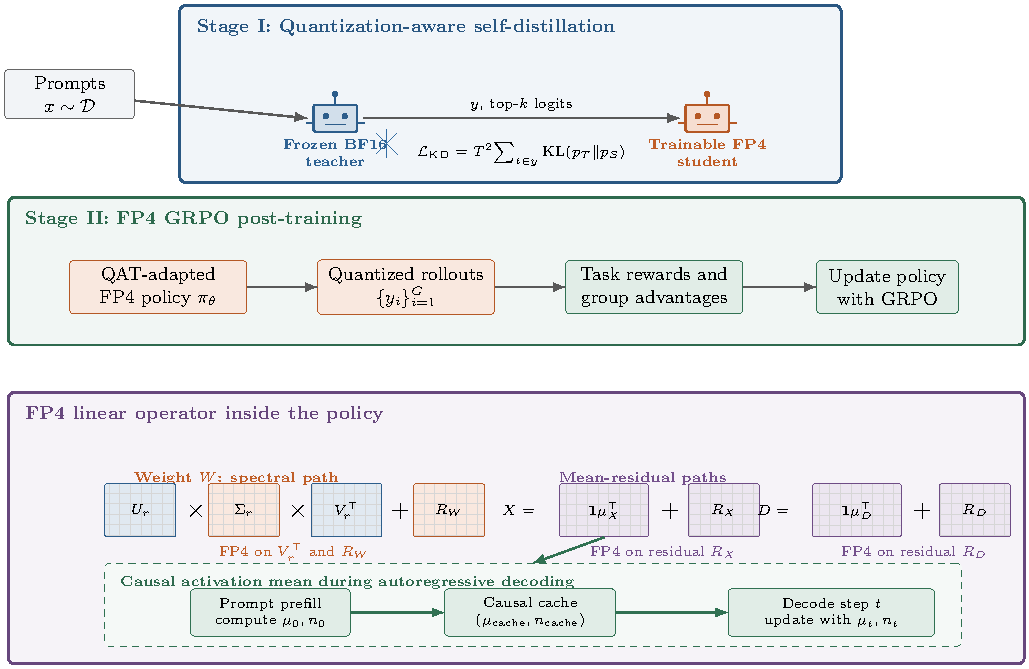
\includegraphics[width=\textwidth]{Figures/fp4_post_training_pipeline.pdf}
    \caption{Two-stage FP4 post-training pipeline. Stage~I freezes the BF16 teacher $\pi_T$ and updates $\pi_\theta$ by masked token-level distillation. Stage~II uses the adapted $\pi_\theta$ to generate rollouts, compute task rewards and group-relative advantages, and perform GRPO updates. Mean NVFP4 quantizes $U_r$, $V_r^\top$, and $R_W$ while retaining $\Sigma_r$ in higher precision. Activations and output gradients are centered before their residuals are quantized, and a causal activation-mean cache supplies the decode-time mean.}
    \label{fig:pipeline}
\end{figure*}

Let $\widehat A_i$ denote the group-relative advantage obtained by normalizing task rewards within a group of $G$ completions, and let $\rho_i(\theta)=\pi_\theta(y_i\mid x)/\pi_{\mathrm{old}}(y_i\mid x)$. For compactness, the following equation is a sequence-level abstraction of the implemented token-level objective, which forms ratios over valid completion tokens:
\begin{equation}
\begin{aligned}
\mathcal{L}_{\mathrm{GRPO}}(\theta)
&= -\frac{1}{G}\sum_{i=1}^{G}
\min\!\bigl(\rho_i(\theta)\widehat A_i, \\[-0.2ex]
&\hspace{2.2cm}\operatorname{clip}(\rho_i(\theta),1-\epsilon,1+\epsilon)\widehat A_i\bigr).
\end{aligned}
\end{equation}
In FP4 GRPO, quantization error also changes sampled trajectories and therefore the task rewards and group-relative advantages used for subsequent updates.

The frozen teacher $\pi_T$ uses BF16 linear layers. For the trainable policy $\pi_\theta$, master parameters remain in higher precision, while each selected linear projection is evaluated with FP4 operands in the forward and backward matrix multiplications. The sampling-time policy $\pi_{\mathrm{old}}$ uses the same quantized forward path as $\pi_\theta$ at rollout generation. We apply a fixed weight-decomposition path and FP4 quantization to weights, activations, and gradients; the activation and gradient quantization paths define the experimental condition.

\subsection{Spectral Weight Factorization}

Before post-training, we decompose each selected weight matrix $W\in\mathbb{R}^{d_{\mathrm{out}}\times d_{\mathrm{in}}}$ into a rank-$r$ truncated-SVD approximation and a residual:
\begin{equation}
    W_r = U_r\Sigma_r V_r^{\top},
    \qquad
    R_W = W-W_r,
    \qquad
    W=W_r+R_W,
    \label{eq:weight-svd}
\end{equation}
where $U_r\in\mathbb{R}^{d_{\mathrm{out}}\times r}$, $\Sigma_r\in\mathbb{R}^{r\times r}$, and $V_r\in\mathbb{R}^{d_{\mathrm{in}}\times r}$. Metis uses this split because a few singular components can dominate the dynamic range \citep{cao2025metis}. We use $r=64$ and quantize the low-rank factors and residual with separate NVFP4 operators; $\Sigma_r$ remains in higher precision. Denoting NVFP4 quantize--dequantize by $Q_{\mathrm{NVFP4}}$, the effective weight is
\begin{equation}
    \widetilde W
    = Q_{\mathrm{NVFP4}}(U_r)\Sigma_r
      Q_{\mathrm{NVFP4}}(V_r^{\top})
      + Q_{\mathrm{NVFP4}}(R_W).
    \label{eq:weight-reconstruct}
\end{equation}
For a row-major activation matrix $X$, the forward GEMM is $Y=\widehat X\widetilde W^{\top}+b$. The implementation first applies the NVFP4-quantized $V_r^{\top}$ projection, scales the rank-$r$ features by the higher-precision $\Sigma_r$, projects them with NVFP4-quantized $U_r$, and adds the NVFP4-quantized residual branch. The low-rank and residual branches therefore use separate NVFP4 scales.

\subsection{Mean NVFP4}

Mean NVFP4 centers activations and output gradients around their feature-wise means before quantizing the residuals. Let $X\in\mathbb{R}^{L\times d_{\mathrm{in}}}$ denote a flattened activation matrix, where $L$ merges batch and sequence positions. Following the mean-bias observation of Averis \citep{cao2026averis}, we isolate the feature-wise mean
\begin{equation}
    \mu_X = \frac{1}{L}\mathbf{1}_L^{\top}X,
    \qquad
    X_R = X-\mathbf{1}_L\mu_X,
    \label{eq:activation-split}
\end{equation}
and apply FP4 only to the centered residual:
\begin{equation}
    \widehat X
    = \mathbf{1}_L\mu_X+Q_{\mathrm{NVFP4}}(X_R).
    \label{eq:activation-qdq}
\end{equation}
Mean NVFP4 restores the shared offset in higher precision after quantizing the centered residual. Centering allocates the finite FP4 codebook to token-to-token variation rather than to a coherent rank-one offset. The activation path uses mean-residual quantization in place of activation SVD.

The backward output gradient is treated analogously. For $D=\partial\mathcal{L}/\partial Y\in\mathbb{R}^{L\times d_{\mathrm{out}}}$, define
\begin{equation}
    \begin{aligned}
        \mu_D&=\frac{1}{L}\mathbf{1}_L^{\top}D,
        &D_R&=D-\mathbf{1}_L\mu_D,\\[-0.2ex]
        \widehat D&=\mathbf{1}_L\mu_D+Q_{\mathrm{NVFP4}}(D_R).
    \end{aligned}
    \label{eq:gradient-qdq}
\end{equation}
The low-precision linear backward path then uses
\begin{equation}
    \widehat{\nabla_W\mathcal{L}}=\widehat D^{\top}\widehat X,
    \qquad
    \widehat{\nabla_X\mathcal{L}}=\widehat D\widetilde W.
    \label{eq:quantized-backward}
\end{equation}
Expanding the reconstructed low-precision weight-gradient GEMM yields four terms:
\begin{equation}
    \begin{aligned}
    \widehat{\nabla_W\mathcal{L}}
    ={}& Q_{\mathrm{NVFP4}}(D_R)^{\top}Q_{\mathrm{NVFP4}}(X_R)
    + Q_{\mathrm{NVFP4}}(D_R)^{\top}\mathbf{1}_L\mu_X \\[-0.2ex]
    &+ \mu_D^{\top}\mathbf{1}_L^{\top}Q_{\mathrm{NVFP4}}(X_R)
    + L\mu_D^{\top}\mu_X.
    \end{aligned}
    \label{eq:mean-gradient-identity}
\end{equation}
Because quantize--dequantize residuals and masked reductions are not guaranteed to be zero mean, the implementation retains all four terms in Eq.~\ref{eq:mean-gradient-identity}.

During prompt prefill, the method computes $\mu_X$ over all available prompt positions and stores both the mean and the number of represented token positions. At autoregressive decode step $t$, let $\mu_t$ be the mean of the newly observed positions and $n_t$ their count. The cache is updated as
\begin{equation}
    \mu_{\mathrm{cache}} \leftarrow
    \frac{n_{\mathrm{cache}}\mu_{\mathrm{cache}}+n_t\mu_t}
    {n_{\mathrm{cache}}+n_t}.
    \label{eq:causal-mean-cache}
\end{equation}
At decode time, Eq.~\ref{eq:activation-qdq} uses $\mu_{\mathrm{cache}}$ in place of $\mu_X$. This construction does not access future generated tokens. A full-sequence training forward and a prefix-only decode forward can nevertheless use different means, producing a train--decode mismatch in the current estimator.

\subsection{Mean Self-Distillation Before GRPO}

The proposed pipeline has two stages. First, the frozen BF16 teacher $\pi_T$ samples a response $y$ for each prompt $x$. The teacher $\pi_T$ and trainable low-precision policy $\pi_\theta$ then perform full forwards on the same concatenated sequence $(x,y)$. Let $z_{M,b,t,v}$ denote the next-token logit of model $M\in\{T,\theta\}$ for vocabulary item $v$ at response position $t$ in minibatch example $b$. We select the teacher's top-$k$ set and renormalize both models over that same set:
\begin{equation}
\begin{aligned}
\mathcal{K}_{b,t}
&=\operatorname{TopK}_k\!\left(z_{T,b,t,\cdot}\right),\\
\widetilde p_{M,b,t}(v)
&=\frac{\exp(z_{M,b,t,v}/T)}
{\sum_{u\in\mathcal{K}_{b,t}}\exp(z_{M,b,t,u}/T)},
\quad v\in\mathcal{K}_{b,t}.
\end{aligned}
\end{equation}

Let $m_{b,t}\in\{0,1\}$ indicate a valid response token and let $N_{\mathrm{valid}}=\sum_{b,t}m_{b,t}$. The implemented objective is
\begin{equation}
\begin{aligned}
\mathcal{L}_{\mathrm{KD}}
=\frac{T^2}{\max(N_{\mathrm{valid}},1)}
\sum_{b,t}m_{b,t}
\sum_{v\in\mathcal{K}_{b,t}}
\widetilde p_{T,b,t}(v)
\log\frac{\widetilde p_{T,b,t}(v)}
{\widetilde p_{\theta,b,t}(v)}.
\end{aligned}
\label{eq:topk-distillation}
\end{equation}
By default, $k=100$. We retain only the teacher's top-$k$ logits and indices and gather the corresponding logits from $\pi_\theta$. Both distributions are renormalized over the teacher-selected subset, and the loss is averaged over all valid response tokens in the minibatch. Mean self-distillation thereby adapts the low-precision computation path of $\pi_\theta$ to the teacher's dominant response distribution before the policy is used to explore and optimize task rewards. In the second stage, the adapted $\pi_\theta$ is trained with GRPO on DeepMath-103K examples using a binary mathematical-equivalence task reward.

\begin{algorithm}[t]
\caption{Mean Self-Distillation Followed by FP4 GRPO}
\begin{algorithmic}[1]
\STATE Initialize frozen BF16 teacher $\pi_T$ and trainable FP4 policy $\pi_\theta$ from the same base checkpoint.
\FOR{each Mean self-distillation minibatch of prompts $x$}
    \STATE Sample teacher responses $y\sim\pi_T(\cdot\mid x)$.
    \STATE Update $\pi_\theta$ with the masked, top-$k$-normalized distillation loss $\mathcal{L}_{\mathrm{KD}}$.
\ENDFOR
\FOR{each GRPO minibatch of prompts $x$}
    \STATE Sample quantized rollouts $\{y_i\}_{i=1}^{G}$ from $\pi_\theta$ and denote this sampling-time policy by $\pi_{\mathrm{old}}$.
    \STATE Compute task rewards and group-relative advantages.
    \STATE Update $\pi_\theta$ with the GRPO objective using probability ratios relative to $\pi_{\mathrm{old}}$.
\ENDFOR
\end{algorithmic}
\end{algorithm}

\FloatBarrier

\section{Experiments}

\subsection{Models, Data, and Baselines}

The study post-trains Qwen2.5-0.5B-Instruct \citep{yang2024qwen25}, Qwen2.5-Math-1.5B-Base, and Qwen2.5-Math-7B-Base \citep{yang2024qwen25math} on DeepMath-103K \citep{he2025deepmath}, a collection of 103,022 mathematical problems curated for RL and supervised fine-tuning. The dataset provides a final answer for each problem, which we use to compute rule-based task rewards. Mean self-distillation uses teacher-generated responses on the same prompt distribution.

The downstream comparison includes the initial checkpoint as an evaluation reference, completed BF16 GRPO and Mean NVFP4 GRPO checkpoints, NVFP4 GRPO runs that fail during training, and the Hadamard NVFP4 GRPO baseline.

We evaluate each reported checkpoint with EvalScope on AIME 2024, AIME 2025, the AMC 2022--2024 split, MATH-500 \citep{lightman2023letsverify}, ARC \citep{clark2018arc}, and GPQA-Diamond \citep{rein2023gpqa}. EvalScope uses its task-specific answer extraction and accuracy scorer. Each prompt receives one completion with \texttt{do\_sample=false}, temperature 0, \texttt{top\_k=0}, \texttt{top\_p=1.0}, and at most 2048 new tokens. Mean NVFP4 checkpoints are evaluated with native NVFP4 inference rather than the simulated training operator. The current run metadata does not retain the EvalScope version.

\subsection{Training Protocol}

Table~\ref{tab:protocol} gives the default Qwen2.5-0.5B-Instruct diagnostic protocol. Runs within each reported comparison use the same DeepMath-103K split, task-reward implementation, prompt order, generation limits, and GRPO budget.

\begin{table*}[!t]
\centering
\small
\caption{Default controlled diagnostic protocol for Qwen2.5-0.5B-Instruct. Mean self-distillation and GRPO step budgets are set explicitly for each reported run.}
\label{tab:protocol}
\begin{tabular}{@{}p{0.17\textwidth}p{0.37\textwidth}p{0.37\textwidth}@{}}
\toprule
Setting & Mean self-distillation & GRPO post-training \\
\midrule
Data & \multicolumn{2}{l}{DeepMath-103K training split; identical prompt order within each seed} \\
Precision & frozen BF16 $\pi_T$; trainable FP4 $\pi_\theta$ forward/backward & higher-precision master parameters; FP4 $\pi_\theta$ forward/backward \\
Batching & 16 prompts/GPU; accumulation 4 & 64 prompts/GPU; accumulation 1; $G=8$ completions/prompt \\
Sequence limits & prompt 512; teacher generation 1024 & prompt 1024; completion 1024 \\
Optimization & AdamW, learning rate $10^{-6}$, 5\% warmup, gradient norm 1.0 & AdamW, learning rate $10^{-6}$, gradient norm 1.0 \\
Training objective & $T=1$, one teacher response/prompt, top-$k=100$ distillation & clipped GRPO with group-relative advantages normalized within each prompt group \\
Task reward & --- & binary exact-match/equivalence task reward \\
Generation & --- & cache enabled; gradient checkpointing enabled \\
Quantized paths & weights: rank-64 factorization; activations/output gradients: centered-residual NVFP4 & NVFP4: direct weight/activation/gradient QDQ; Hadamard NVFP4: Hadamard-preconditioned weights and weight-gradient operands, direct remaining paths; Mean NVFP4: rank-64 weight factorization and centered-residual activations/output gradients \\
Weight rank & 64 & 0 for NVFP4 and Hadamard NVFP4; 64 for Mean NVFP4 \\
\bottomrule
\end{tabular}
\end{table*}

\subsection{Rollout Diagnostics}

The completion-level diagnostics record empty or short output, non-printable-character ratio, repeated $n$-grams, consecutive token loops, lexical diversity, punctuation and symbol ratios, and language switching. Token-level logs contain rollout probability summaries. Step-level aggregates include the bad-rollout rate, task-reward statistics, activation summaries, and separate trends for responses classified as good or bad. The bad-rollout labels are multi-label, so one completion can receive more than one failure label.

\section{Results}

\subsection{Logged Rollout Diagnostics Before and After Mean Self-Distillation}
\label{sec:mean-self-distillation-analysis}

Figure~\ref{fig:nvfp4-bad-types} breaks the aggregate NVFP4 bad-rollout rate into diagnostic labels. Low lexical diversity and token loops account for many flagged completions; short output and language switching also occur. Because the labels are assigned independently, their proportions need not sum to one. The labels show which visible failure modes contribute to the aggregate bad-rollout rate. They do not isolate every source of task-reward change.

\begin{figure}[!t]
    \centering
    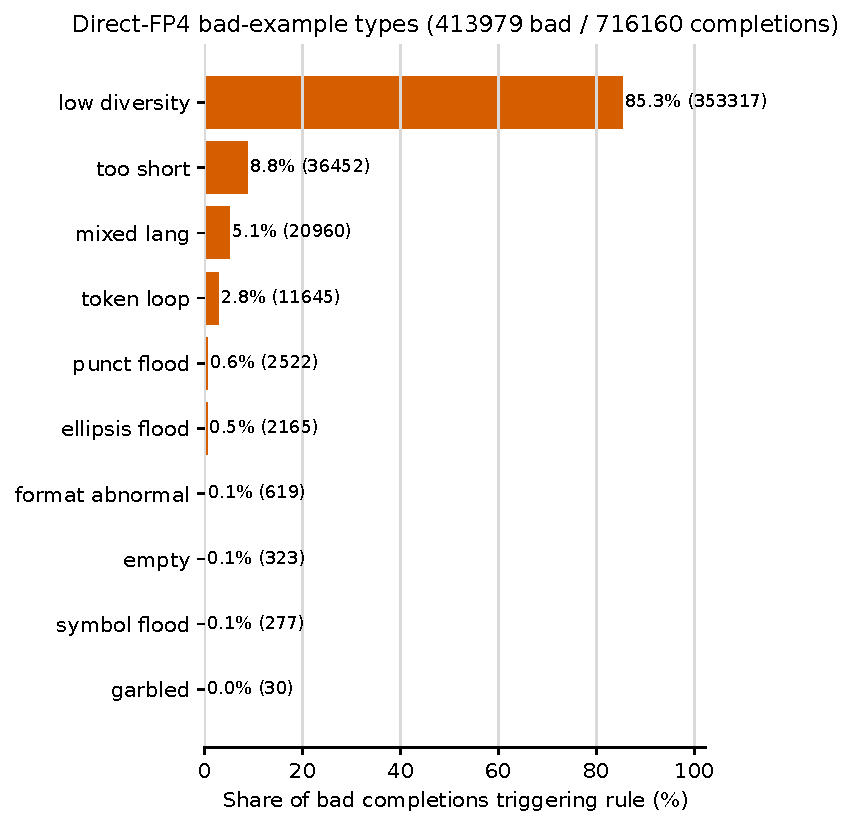
\includegraphics[width=0.92\linewidth]{Figures/direct_fp4_bad_types_qwen_0_5b.pdf}
    \caption{Multi-label composition of NVFP4 bad rollouts for Qwen2.5-0.5B-Instruct. A completion can receive more than one failure label.}
    \label{fig:nvfp4-bad-types}
\end{figure}

Figure~\ref{fig:bad-rollout-trajectory} compares NVFP4 GRPO with Mean NVFP4 GRPO after Mean self-distillation in one Qwen2.5-0.5B-Instruct run. The full two-stage configuration has a lower bad-rollout rate over the logged steps. This comparison is descriptive because it contains one run per condition.

\begin{figure}[!t]
    \centering
    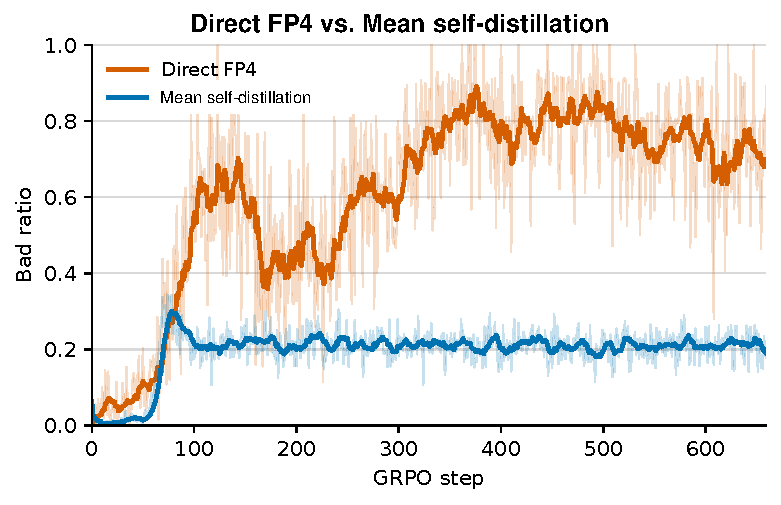
\includegraphics[width=\linewidth]{Figures/rollout_bad_ratio_qwen_0_5b.pdf}
    \caption{Bad-rollout-rate trajectories for Qwen2.5-0.5B-Instruct. NVFP4 is compared with Mean NVFP4 after Mean self-distillation over the logged GRPO steps. Pale traces are logged values and solid traces are trailing averages.}
    \label{fig:bad-rollout-trajectory}
\end{figure}

Figure~\ref{fig:reward-trajectory} reports TensorBoard \texttt{train/reward} over the same logged steps. At 0.5B, the two FP4 runs start at similar logged task-reward levels and end at different values. Matched seeds are needed to determine whether this separation is reproducible. The comparison also changes self-distillation and the Mean NVFP4 quantization path together.

\begin{figure}[!t]
    \centering
    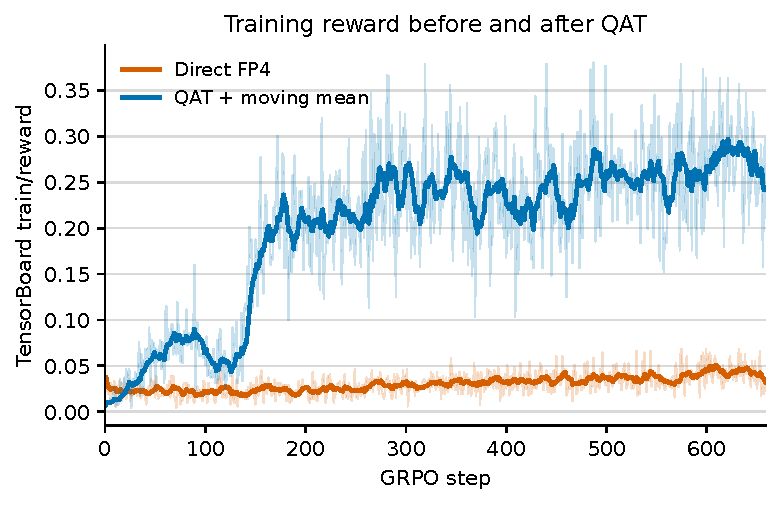
\includegraphics[width=\linewidth]{Figures/rollout_reward_qwen_0_5b.pdf}
    \caption{Mean logged task-reward trajectories for Qwen2.5-0.5B-Instruct. The plot uses TensorBoard \texttt{train/reward}; pale traces are logged values and solid traces are trailing moving averages.}
    \label{fig:reward-trajectory}
\end{figure}

\subsection{Main Results}

Table~\ref{tab:main} reports downstream accuracy. At 1.5B, Mean NVFP4 GRPO improves over the initial checkpoint by 42.2 points on MATH-500 and 55.50 points on ARC, but AIME25 decreases by 3.33 points. Relative to BF16 GRPO, it is 6.0 points lower on AMC, 2.4 points lower on MATH-500, 1.78 points higher on ARC, and 3.03 points lower on GPQA-Diamond. At 7B, Mean NVFP4 GRPO matches BF16 GRPO on MATH-500 and is higher by 3.3, 10.0, and 4.47 points on AIME24, AIME25, and AMC, respectively. It is lower than BF16 GRPO by 18.45 points on ARC and 2.53 points on GPQA-Diamond.

\begin{table*}[!t]
\centering
\footnotesize
\caption{Downstream accuracy (\%) evaluated with EvalScope. ``Initial checkpoint'' denotes the evaluation reference before post-training, and ``Mean NVFP4 GRPO'' denotes Mean self-distillation followed by GRPO with Mean NVFP4. NVFP4 runs that fail before evaluation are marked ``Training failed.''}
\label{tab:main}
\begin{tabular}{llrrrrrr}
\toprule
Model & Method & AIME24 & AIME25 & AMC & MATH-500 & ARC & GPQA-Diamond \\
\midrule
Qwen2.5-0.5B-Instruct & Initial checkpoint & 0.0 & 0.0 & 6.72 & 29.6 & 54.62 & 18.69 \\
& BF16 GRPO & 3.3 & 0.0 & 8.95 & 32.2 & 53.22 & 24.24 \\
& NVFP4 GRPO & \multicolumn{6}{c}{Training failed} \\
& Hadamard NVFP4 GRPO & -- & -- & -- & -- & -- & -- \\
& Mean NVFP4 GRPO & 0.0 & 0.0 & 6.72 & 6.0 & 29.6 & 24.24 \\
\midrule
Qwen2.5-Math-1.5B-Base & Initial checkpoint & 6.67 & 10.0 & 20.15 & 25.8 & 7.89 & 0.51 \\
& BF16 GRPO & 13.3 & 3.3 & 38.8 & 70.4 & 61.61 & 22.73 \\
& NVFP4 GRPO & \multicolumn{6}{c}{Training failed} \\
& Hadamard NVFP4 GRPO & -- & -- & -- & -- & -- & -- \\
& Mean NVFP4 GRPO & 10.0 & 6.67 & 32.8 & 68.0 & 63.39 & 19.7 \\
\midrule
Qwen2.5-Math-7B-Base & Initial checkpoint & 6.67 & 3.3 & 5.97 & 17.4 & 15.53 & 8.59 \\
& BF16 GRPO & 10.0 & 3.3 & 46.27 & 78.0 & 78.52 & 33.84 \\
& NVFP4 GRPO & \multicolumn{6}{c}{Training failed} \\
& Hadamard NVFP4 GRPO & -- & -- & -- & -- & -- & -- \\
& Mean NVFP4 GRPO & 13.3 & 13.3 & 50.74 & 78.0 & 60.07 & 31.31 \\
\bottomrule
\end{tabular}
\end{table*}

\FloatBarrier

The 0.5B model does not show the downstream gains observed at 1.5B and 7B. Relative to its initial checkpoint, Mean NVFP4 GRPO is 23.6 points lower on MATH-500 and 25.02 points lower on ARC; its GPQA-Diamond score increases by 5.55 points and matches BF16 GRPO. The effects are therefore model- and task-dependent.

\section{Conclusion}

Evaluation of FP4 RL post-training should include rollout quality because the policy generates the trajectories used for its own updates. In our pipeline, Stage~I fits the low-precision policy to BF16 teacher logits on teacher-generated prefixes before on-policy updates begin. Stage~II applies GRPO with Mean NVFP4 and a causal activation-mean cache.

NVFP4 GRPO fails to complete training at all three evaluated scales. In the single logged 0.5B comparison, the full two-stage configuration has fewer flagged rollouts and a higher mean logged task reward over the observed steps. Downstream accuracy remains mixed: the 0.5B model declines on MATH-500 and ARC, and the 7B model trails BF16 GRPO on ARC. Rollout diagnostics complement fixed-batch numerical error and downstream accuracy when evaluating an FP4 policy.

The causal activation-mean cache can produce different means from a full-sequence training forward. The rule-based rollout classifier detects visible degeneration, not semantic correctness. The current comparisons also change self-distillation, weight decomposition, and centering together, so they do not isolate each component, and seed-level uncertainty is not reported. Reproducible comparisons require the quantization recipe, decoding configuration, software and hardware versions, EvalScope version, and per-seed results.

\bibliography{fp4_post_aaai_draft}
\end{document}
